%% The following is a directive for TeXShop to indicate the main file
%%!TEX root = diss.tex

\chapter{A new taxonomy of 3D Reconstruction}
\label{ch:3DRecon_Taxo}
Existing taxonomies of 3D reconstruction techniques generally only focus on one category of techniques: ~\citeauthor{seitz2006comparison} proposed  multiple means to classify Multi-view Stereo algorithms from various perspectives. Reviews \cite{geng2011structured, salvi2004pattern} of Structured Light techniques generally classify techniques based on the type of projection pattern used. Photometric Stereo algorithms are classified by the assumptions or generalizations made, for instance, calibrated/uncalibrated, unknown/known reflectance, unknown/known light conditions, etc. This framework provides a means to categorize intra-category algorithms, but is unsuitable to evaluate the performance of each technique across object with a range of attributes.

To have a more comprehensive understanding of the strengths and weaknesses of different techniques, a more general taxonomy is need, and one of the most popular framework categorizes 3D reconstruction techniques into active and passive methods: if the controlled light condition is used, then it's active, otherwise, it's passive. Other notable taxonomy is the spacetime framework proposed in \cite{davis2003spacetime}, which categorizes depth from triangulation techniques based on the sources of information: temporal or spatial information. Though widely adopted, the mapping of the algorithm to the conditions that works the best is generally empirical.

In the previous taxonomies, algorithms of a certain category generally work well on limited conditions, and a it's crucial to understand where algorithms perform well and where they fail. Under the previous framework, this knowledge is largely empirical, with each algorithm roughly maps to a problem domain that is poorly defined.

The taxonomy proposed in this chapter defines the 3D reconstruction techniques from a object-centered viewpoint, \ie categorize algorithm based on object class. This taxonomy transforms the 3D reconstruction problem from one requiring knowledge and expertise of specific algorithms in terms of how and when to use them, to one requiring knowledge of the visual and geometric properties of the target object.

We need to way general/univeral enough that incorporates any between-class methods, and distinctive enough that distinguish with-class methods.

\section{Object class}
In Figure~\ref{fig:obj_class}, we show a taxonomy of object classes with different material and shape properties. There are in total $3\times 3\times 4\times 2\times 5 = 360$ classes of objects, which still don't fully capture the variations exhibited by real world objects, for instance, effects such as emission are not considered. Most techniques that have been developed over the past decades have focused on opaque objects with diffuse reflectance. However, the majority of currently available techniques can only tackle a subset of all possible classes. For instance, MVS algorithms typically work well for diffuse texture objects, while there are universally effective algorithms for specular, refractive objects~\cite{ihrke2010transparent}.
\begin{figure}[h]
\centering
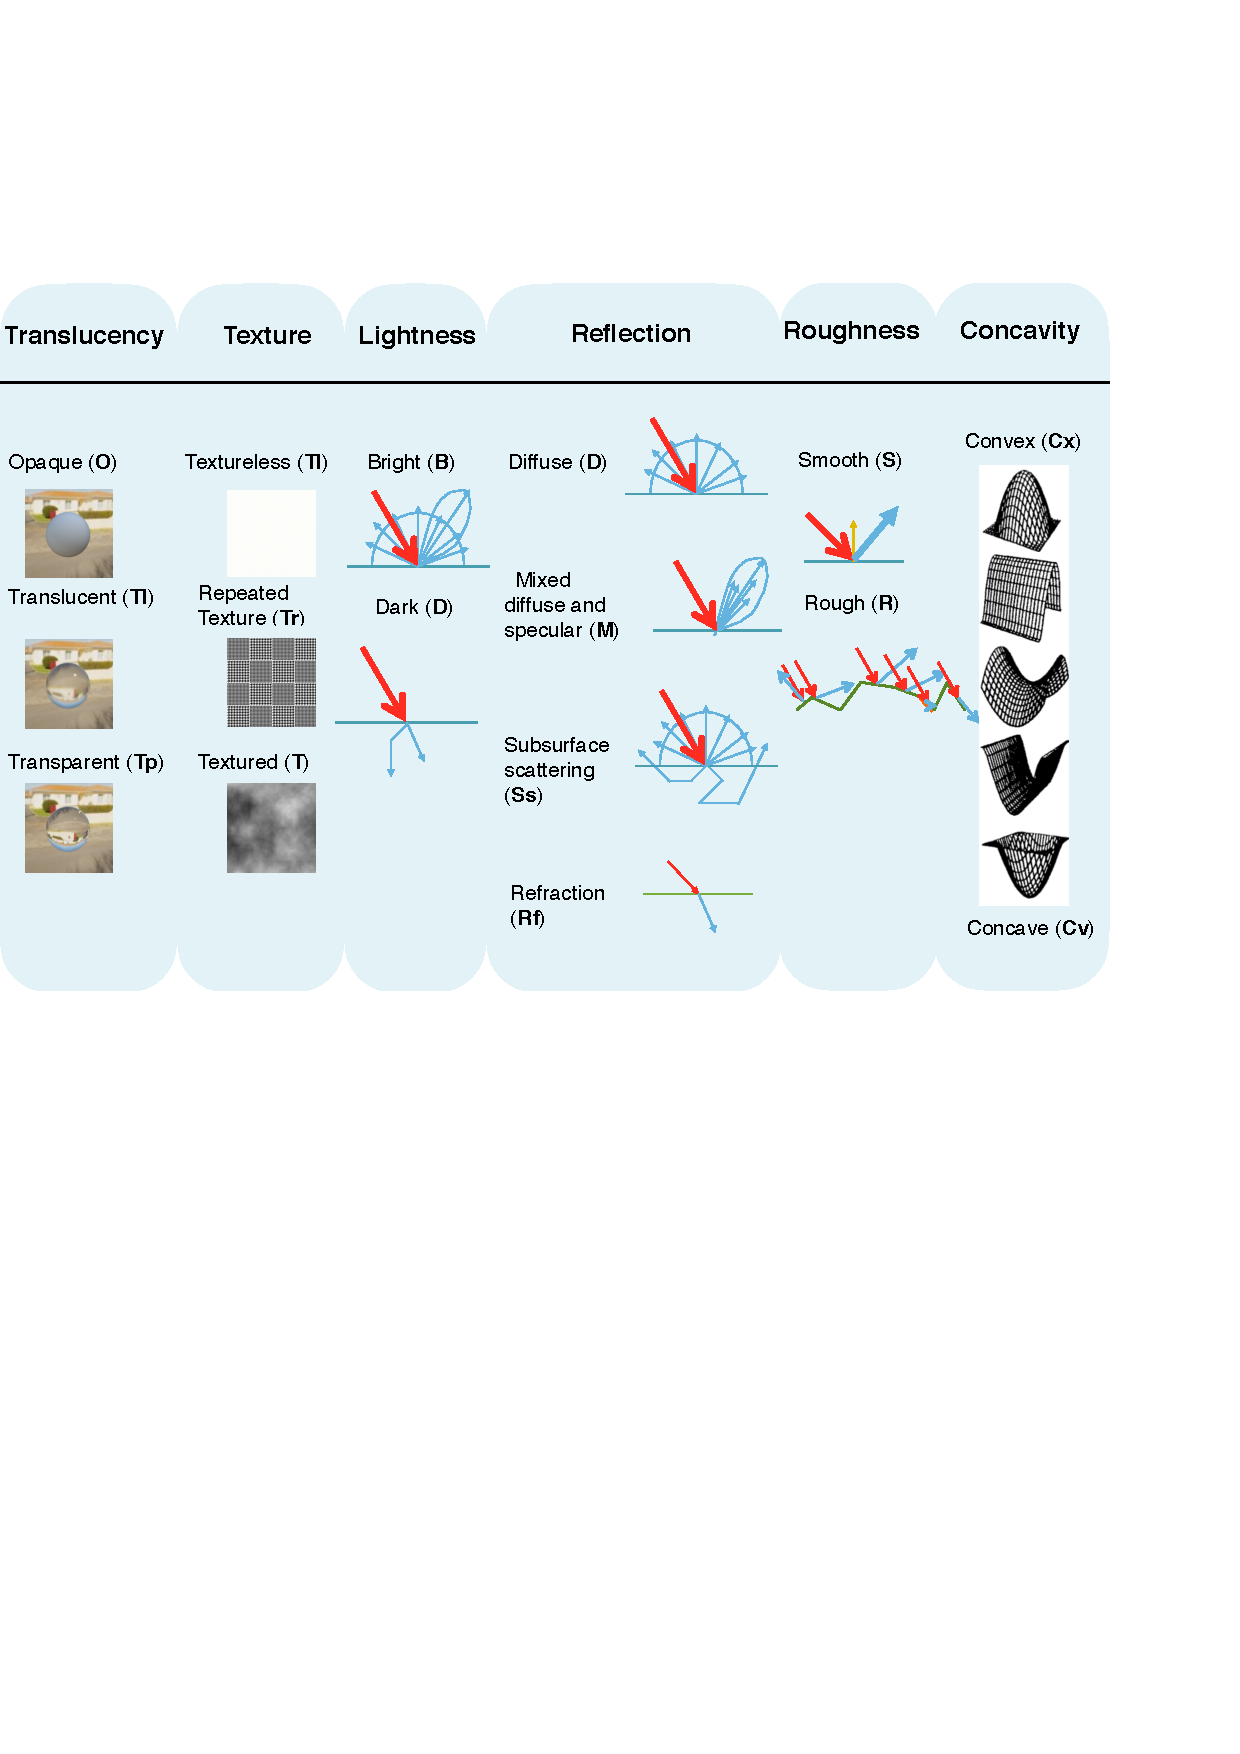
\includegraphics[width=\textwidth]{taxo/obj_class}
\caption{Object class}
\label{fig:obj_class}
\end{figure}

To make the problem tackleable, only four classes of objects are being investigated in depth. The reasoning behind the selected object classes is solely based on the [popularity] of the class. See Figure~\ref{fig:class_of_interest} for the five classes of objects.

\begin{figure}[ht]
\centering
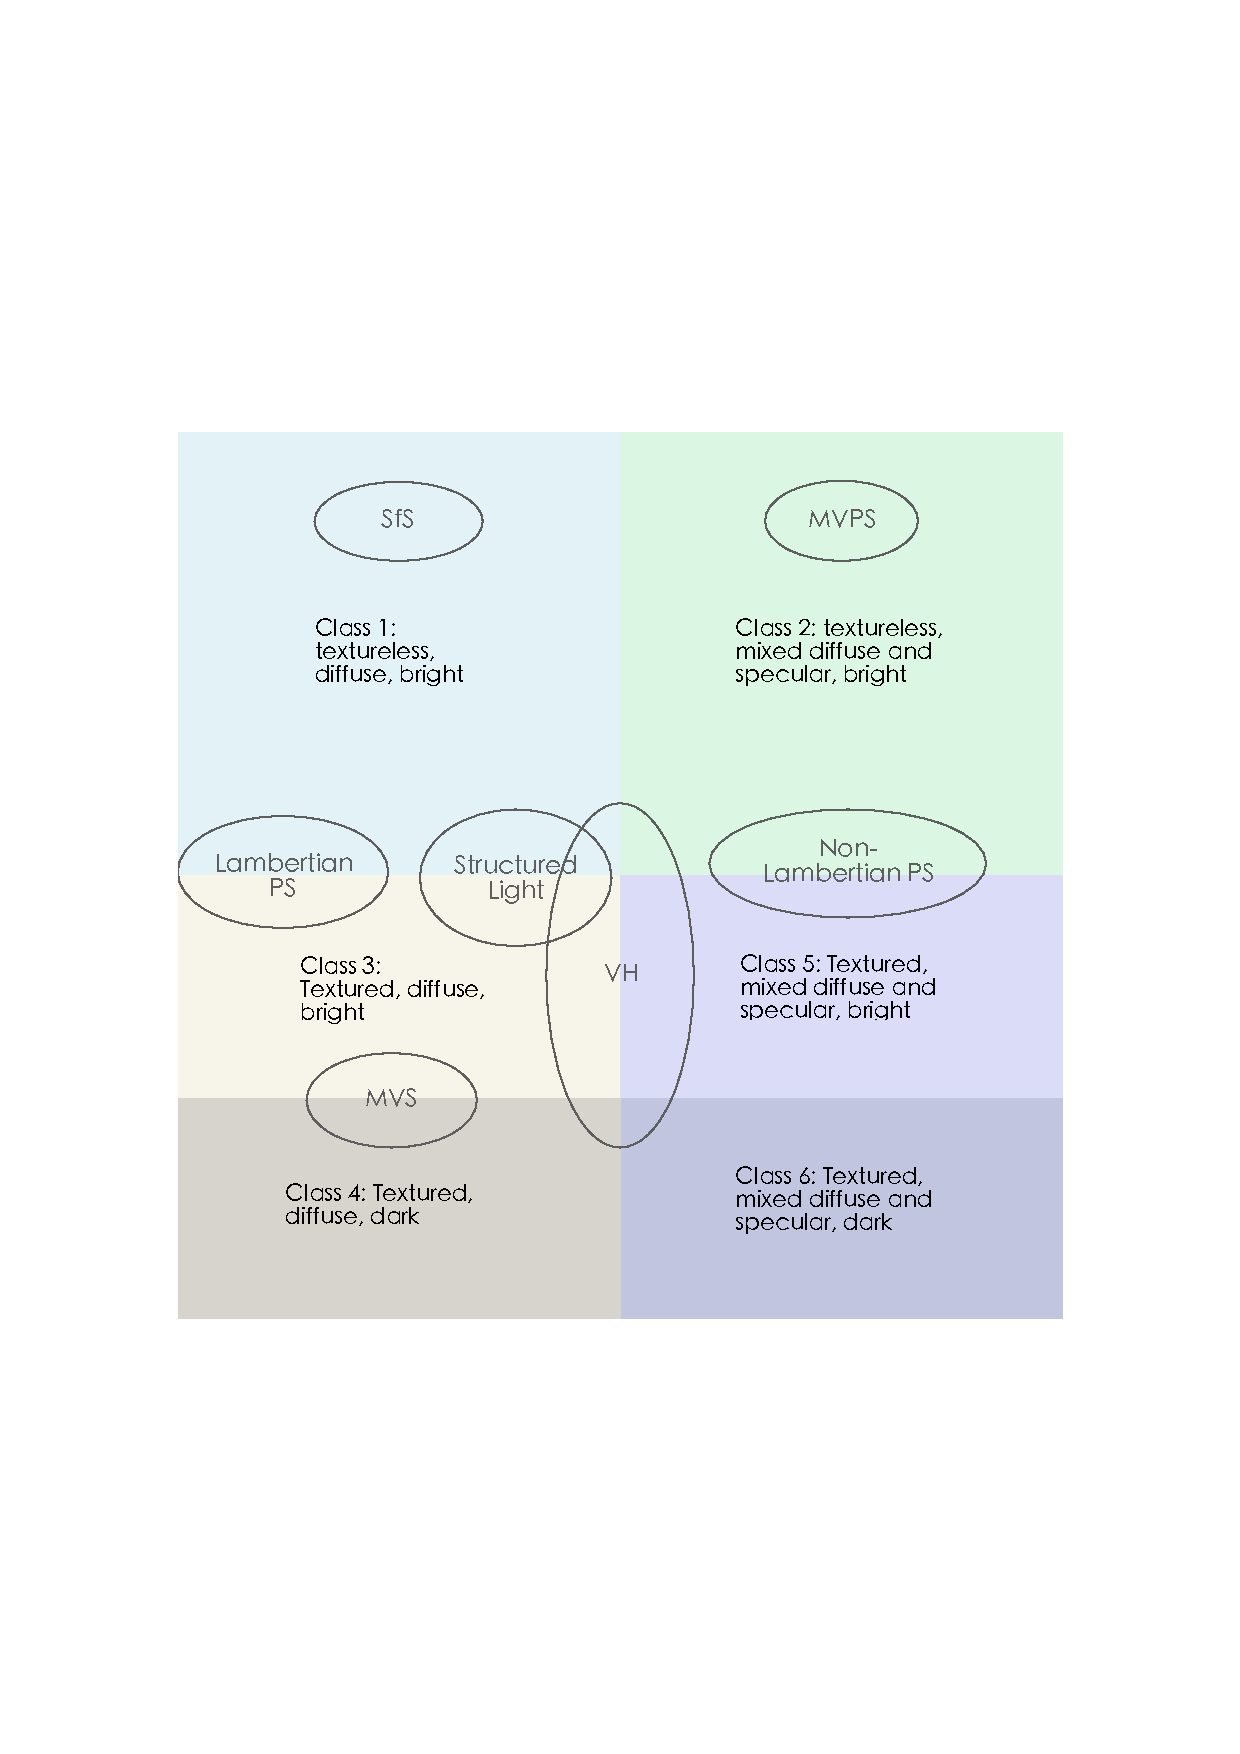
\includegraphics[width=0.6\textwidth]{taxo/six_class}
\caption{Five classes of interest}
\label{fig:class_of_interest}
\end{figure}

Chapter~\ref{ch:RelatedWork} provides an overview of the state-of-the-art techniques in 3D reconstruction based visual/geometric cues used. However, this fails to provide a context as where the algorithm should be used.

\section{Class 1}
In this section, we discuss techniques for reconstructing textureless, diffuse, and bright surfaces. The reconstruction of surface is complicated by the fact that there is no spatial information available for stereo correpondence searching due to lack of texture. Furthermore, for specular surfaces reflect light in a single direction which follows the law of reflection, thus the appearance changes as the viewpoint changes, which makes the correspondence search in these regions unreliable.

\begin{table}[h]
  \centering
  \begin{tabular}{l*{2}{c}}
  \hline
  \textbf{Reference} & Reflectance & Calibrated \\
  \hline
  Horn~\cite{horn1989shape} & Lambertian & Yes\\
  Woodham~\cite{woodham1980photometric} & Lambertian & Yes\\
  \hline
  \end{tabular}
  \caption{Summary of Lambertian Photometric Stereo assumptions and formulations}
  \label{tab:class_1}
\end{table}

\subsection{Shape from Shading}
The technique of shape from shading estimates surface orientation from shading variations. As discussed in Chapter~\ref{ch:RelatedWork}, the radiance depends on the reflectance, lighting and viewing direction, and surface orientation. By assuming known, isotropic surface reflectance, orthographic projection, and known magnitude and direction of the light source, pixel intensity $I(x, y)$ is directly related to surface orientation. This relation is encoded by the reflectance map $R(p, q)$, \ie iso-intensity curves in the gradient space. The problem thus becomes:
$$
I(x, y) = R(p, q)
$$

Unfortunately, measurements of the brightness at a single pixel only provide one constraint whereas surface orientation requires two. All we know is that the surface orientation that has produced $I(x, y)$ lies somewhere on a contour of $R(p, q)$. Additional constaints are needed to estimate the surface orientations.

\subsection{Lambertian Photometric Stereo}
Lambertian Photometric Stereo deals with surfaces with Lambertian reflectance, \ie the emittant radiance in all directions are the same, thus leading to the brightness/colour constancy.

\subsubsection{Calibrated Photometric Stereo}
The original Photometric Stereo, introduced by \citeauthor{woodham1980photometric} overcame the challenges faced by Shape from Shading techniques by adding multiple light sources with different directions. The proposed method deals with Lambertian surfaces, and assumes that the light intensity and direction are known.

This approach not only can estimate surface orientation, but also surface reflectance, \ie spatially varying albedo. Recall the albedo-scaled normal matrix $N_{P\times 3}$ from Chapter~\ref{ch:RelatedWork}, the albedo and surface normal are estimated by
% $$
% I=N^\top L
% $$
% thus the surface normals can be estimated as
% $$
% N = IL^+
% $$
% where $L^+$ is the pseduo-inverse of $L$. The per-pixel albedo and surface normal are
\begin{align*}
\rho_i &= \|N_{i,:}\|\\
n_i &= \frac{N_{i,:}^\top}{\|N_{i,:}\|}
\end{align*}

\subsection{Uncalibrated Photometric Stereo}
It's possible to estimate the surface orientation without knowing the light directions, a case known as \textit{uncalibrated Photometric Stereo}. Most such techniques assume Lambertian techniques and are based on factorization technique proposed in \cite{hayakawa1994photometric}. Recall the Irradiance equation from Chapter~\ref{ch:RelatedWork}
$$
I=N^\top L
$$
However, an infinite number of candidates $\hat{N}$ and $\hat{L}$ make the above equality met. In fact, any invertible $3\times 3$ matrix $W$ defines a candidate pair $\hat{N} = N\cdot W, \hat{L}=W^{-1}L$. Thus the normal $N$ and light source direction $L$ can only be recovered up to a linear transformation.

\citeauthor{hayakawa1994photometric} proposed to use six or more pixels with the same albedo, and was able to solve for normals up to a rotation ambiguity. It can be further proved that a 3-parameter subset of these transformations, known as the Generalized Bas-Relief (GBR) ambiguity, preserve surface integrability~\cite{belhumeur1999bas}. Thus, given three or more imges of a Lambertian object acquired under light sources of unknown direction and strength, the surface can be reconstructed up to GBR transformation by enforcing surface integrability, see Figure~\ref{fig:gbr} for the effect of GBR-ambiguity.
\begin{figure}[!htbp]
\centering
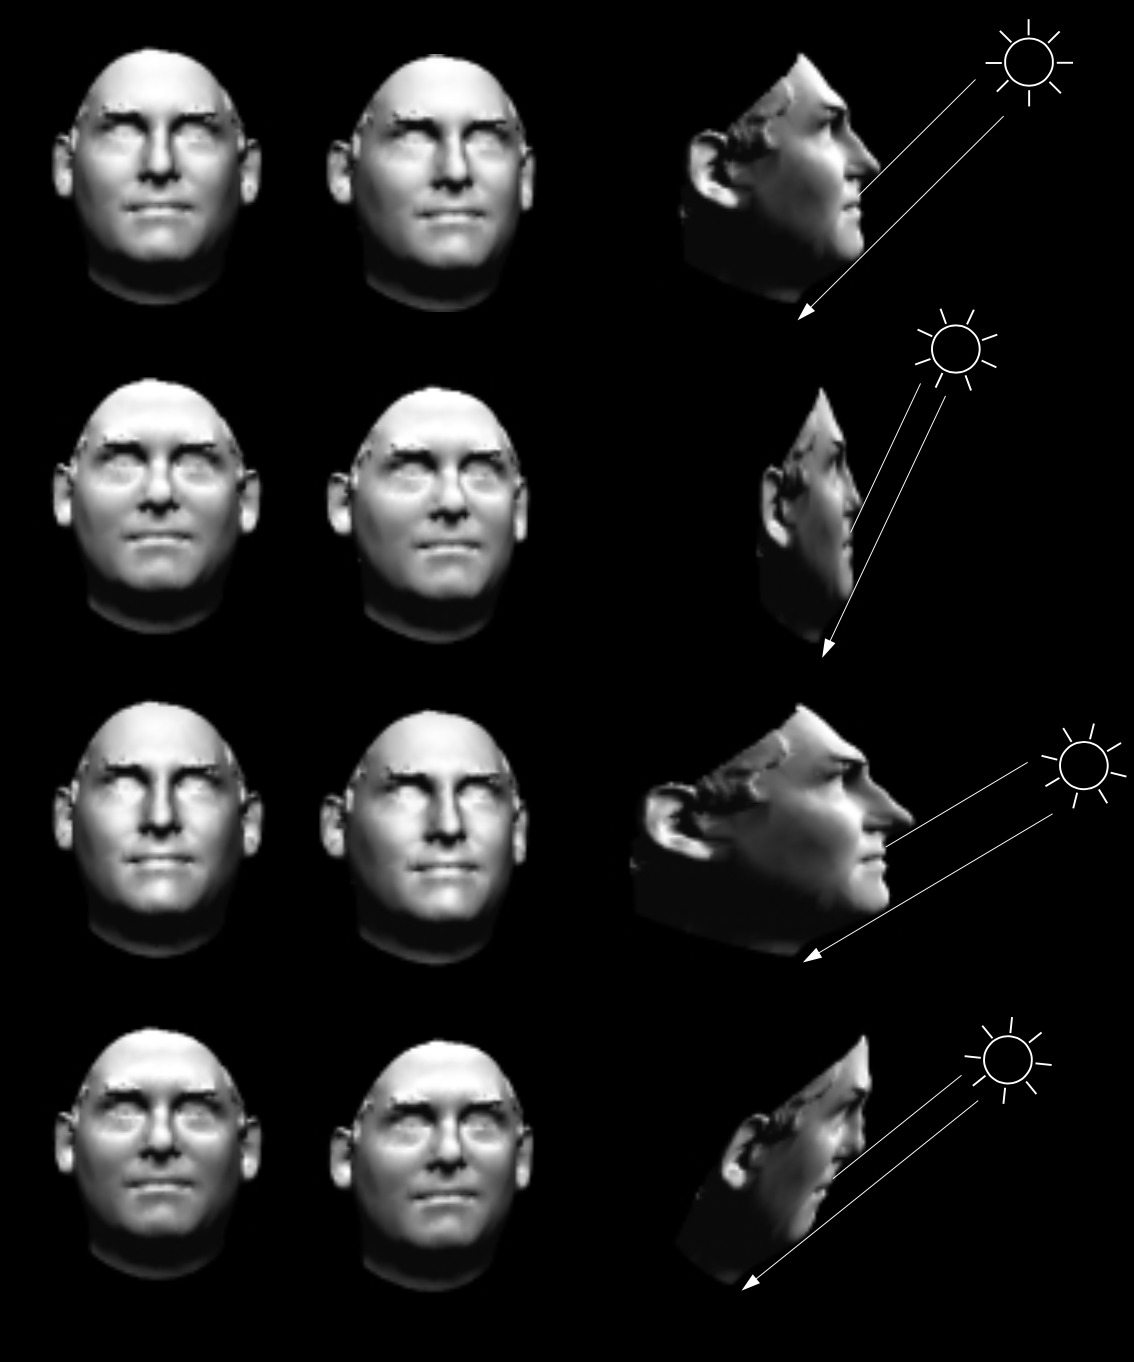
\includegraphics[width=0.6\textwidth]{taxo/gbr.png}
\caption{The effect of GBR ambiguity}
\label{fig:gbr}
\end{figure}

\subsection{Structured Light}
TBW

\section{Class 2}
This section discusses the reconstruction of non-Lambertian, textureless, and bright surfaces. 

\begin{table}[h]
  \centering
  \begin{tabular}{l*{2}{c}}
  \hline
  \textbf{Reference} & Reflectance & Calibrated \\
  \hline
  Coleman~\cite{coleman1982obtaining}, \citeauthor{barsky20034} & specular lobe & Yes\\
  Schluns~\cite{schluns1993photometric}, Sato~\cite{sato1994temporal}, and Mallick~\cite{mallick2005beyond} & specular lobe & Yes\\
  Alldrain~\cite{alldrin2008photometric} & bi-variate function & Yes\\
  Goldman~\cite{goldman2010shape} & Isotropic Ward model & Yes\\
  Silver~\cite{silver1980determining}, Hertzmann~\cite{hertzmann2005example} & reference object(s) & No\\
  Zickler~\cite{zickler2002helmholtz} & physical properties & Yes\\
  \hline
  \end{tabular}
  \caption{Summary of Non-Lambertian Photometric Stereo assumptions and formulations}
  \label{tab:class_2}
\end{table}

\subsection{Non-Lambertian Photometric Stereo}
\subsubsection{Outlier rejection}
One of the research direction in Photometric Stereo is to relax the assumption of Lambertian reflectance. One approach exploits the fact that the reflectance of non-Lambertian surfaces can be approximated by diffuse component and specular lobe. \citeauthor{coleman1982obtaining} and \citeauthor{barsky20034} who treat specular pixels as outliers, and \citeauthor{schluns1993photometric}, \citeauthor{sato1994temporal}, and \citeauthor{mallick2005beyond} who assume the color of the specular lobe differs from the color of the diffuse lobe, allowing separation of the specular and diffuse components.

\subsubsection{Reference objects}
Another research direction uses a reference object that has the same material as the target object. This method is first proposed by~\citeauthor{silver1980determining} and later by~\citeauthor{hertzmann2005example}. Spatially varying BRDF can also be handled by using multiple reference objects, and assuming that the target BRDF is the non-negative linear combination of a set of basis BRDF defined by the set of reference objects.

\subsubsection{Analytic reflectance models}
The idea that BRDF is considered as a non-negative linear combination of basis BRDFs is exploited by~\citeauthor{goldman2010shape}. Their method uses an isotropic Ward model for each basis BRDF, and the surface orientation and parameters of the reflectance models are estimated iteratively. \citeauthor{alldrin2008photometric} proposed a data-driven approach that got rid of the parametric reflectance model, and employed an novel bi-variate approaximations of isotropic reflectance functions. By combining this approximation with the weighted basis BRDFs, a per-pixel surface normal, global set of non-parametric basis BRDFs, and the corresponding weights are able to be independently estimated.

\subsubsection{General properties of a BRDF}
Though the parametric reflectance model can significantly reduce the complexity of BRDFs, they are typically restricted to a limited classes of materials. An alternative is to exploit the physical properties the most materials obey, for instance, Helmholtz reciprocity or isotropy. Helmholtz stereopsis introduced by~\citeauthor{zickler2002helmholtz} exploits the reciprocity to obtain the surface reconstruction.

\subsection{Multi-view Photometric Stereo}


\section{Class 3}
\subsection{Multi-View Stereo}
Multi-view Stereo algorithms reconstruct a (quasi-)dense model by taking advantage of stereo correspondences. We use the following criteria to summarise the MVS algorithms.
\begin{itemize}
\item \textbf{Scene representation}: \textit{3D grid}, \textit{point cloud}, \textit{polygon mesh}, and \textit{depth map};
\item \textbf{Photo-consistency measure}: \textit{scene space}, \textit{image space};
\item \textbf{Visibility model}: \textit{geometric}, \textit{quasi-geometric}, and \textit{outlier-based approach};
\item \textbf{Shape prior}: \textit{minimal surface}, \textit{maximal surface}, and \textit{local smoothness};
\item \textbf{Algorithm}: \textit{extraction from a 3D volume}, \textit{surface/volume evolution}, \textit{seed point propagation}, \textit{per-view depth map reconstruction};
\item \textbf{Initialization}: \textit{bounding box}, \textit{range of depth/disparity}.
\end{itemize}
the We summarize the conditions of these algorithms in Table~
\begin{table}[h]
  \centering
  \begin{tabular}{l*{6}{c}}
  \hline
  \textbf{Technique} & Representation & Photo-consist & Visibility & Shape prior & Algo & Init\\
  \hline
  Furukawa~\cite{furukawa2010accurate} & Point cloud & Scene space, NCC & Quasi-geometry & Seed propagation & N/A\\
  Goesele~\cite{goesele2006multi} & Depth map & Scene space, NCC & Quasi-geomtry & Per-view depth map estimation & Range of depth\\
  Vogiatzis~\cite{vogiatzis2007multiview} \\
  \hline
  \end{tabular}
  \caption{Summary of MVS assumptions and formulations}
  \label{tab:class_3}
\end{table}

\section{Class 4}
\subsection{Visual Hull}

\section{Summary}
Our taxonomy focuses on the visual cues detected in images, which is utilized by various techniques. Conceptualize these visual cues as dimension of the 3D reconstruction problem, we have an abstraction which allow us to think of algorithms as volumes within a $n-$dimensional problem space. Existing algorithms can be introduced into this framework based on the main visual cue used for reconstruction. Instances where these algorithms have been reported as supporting other forms of variation have been outlined, providing an initial mapping of the space that is summarized below in Table~\ref{tab:algo_taxo}.
\begin{sidewaystable}[h]
  \centering
  \begin{tabular}{l*{6}{c}}
  \hline
  \textbf{Technique} & Translucency & Texture & Lightness & Reflectance & Roughness & Concavity\\
  \hline
  Furukawa~\cite{furukawa2010accurate} & Opaque & Textured & N/A & Lambertian & N/A & N/A\\
  Goesele~\cite{goesele2006multi} & Opaque & Textured & N/A & Lambertian & N/A & N/A\\
  Vogiatzis~\cite{vogiatzis2007multiview} & Opaque & Textured & N/A & Lambertian & N/A & N/A\\
  Woodham~\cite{woodham1980photometric} & Opaque & Textureless & Bright & Lambertian & N/A & Convex\\
  Hertzmann~\cite{hertzmann2005example} & Opaque & N/A & Bright & N/A & N/A & Convex\\
  \hline
  \end{tabular}
  \caption{Algorithm classification based on the new taxonomy}
  \label{tab:algo_taxo}
\end{sidewaystable}
